\let\negmedspace\undefined
\let\negthickspace\undefined
\documentclass[journal]{IEEEtran}
\usepackage[a5paper, margin=10mm, onecolumn]{geometry}
\usepackage{lmodern} % Ensure lmodern is loaded for pdflatex
\usepackage{tfrupee} % Include tfrupee package

\setlength{\headheight}{1cm} % Set the height of the header box
\setlength{\headsep}{0mm}     % Set the distance between the header box and the top of the text

\usepackage{gvv-book}
\usepackage{gvv}
\usepackage{cite}
\usepackage{amsmath,amssymb,amsfonts,amsthm}
\usepackage{algorithmic}
\usepackage{graphicx}
\usepackage{textcomp}
\usepackage{xcolor}
\usepackage{txfonts}
\usepackage{listings}
\usepackage{enumitem}
\usepackage{mathtools}
\usepackage{gensymb}
\usepackage{comment}
\usepackage[breaklinks=true]{hyperref}
\usepackage{tkz-euclide} 
\usepackage{listings}
\usepackage{gvv}                                        
\def\inputGnumericTable{}                                 
\usepackage[latin1]{inputenc}                                
\usepackage{color}                                            
\usepackage{array}                                            
\usepackage{longtable}                                       
\usepackage{calc}                                             
\usepackage{multirow}                                         
\usepackage{hhline}                                           
\usepackage{ifthen}                                           
\usepackage{lscape}
\begin{document}

\bibliographystyle{IEEEtran}
\vspace{3cm}

\title{9.7.13}
\author{EE24BTECH11003 - Akshara Sarma Chennubhatla}
% \maketitle
% \newpage
% \bigskip
{\let\newpage\relax\maketitle}
\textbf{Question:}
Solve the differential equation $\frac{dy}{dx} + y \cot x = 4x \cosec x$, with the point $\brak{\frac{\pi}{2}, 0}$ lying on the graph\\

\solution\\
\textbf{Theoretical Solution:}\\

\begin{align}
	\frac{dy}{dx} + y \cot x &= 4x \cosec x\\
\end{align}
This is a linear differential equation. So the Integrating factor is,
\begin{align}
	I.F &= e ^ {\int{\cot x}}\\
	I.F &= e ^ {\log\sin x}\\
	I.F &= \sin x\\
\end{align}
Multiplying both sides of the equation by the integrating factor and integrating,
\begin{align}
	\int{\sin x\brak{\frac{dy}{dx} + y\cot x}} dx &= \int{\sin x 4x \cosec x} dx\\
	y \sin x &= \int{4x} dx\\
	y \sin x &= 2 x^2 + C\\
\end{align}
Since $\brak{\frac{\pi}{2}, 0}$ satisfies the function,
\begin{align}
	0 \brak{1} &= 2 \brak{\frac{\pi}{2}}^2 + C\\
	\implies C &= -\frac{\pi^2}{2}\\
\end{align}
So the function $y\brak{x}$ is,
\begin{align}
	y \sin x &= 2x^2 - \frac{\pi^2}{2}\\
	\implies y &= \frac{2x^2}{\sin x} - \frac{\pi^2}{2\sin x}\\
\end{align}

\textbf{Simulated Solution:}\\

By first principle of derivatives,
\begin{align}
	y^{\prime}\brak{x} = \lim_{h\to 0}\frac{y\brak{x+h} - y\brak{x}}{h}\\
	y\brak{x+h} = y\brak{x} + hy^{\prime}\brak{x}
\end{align}

Given differential equation can be written as,
\begin{align}
	y^{\prime} = 4x \cosec x - y\cot x
\end{align}

So, by using the method of finite diffferences,
\begin{align}
	y_1 = y_0 + h \brak{4x_0 \cosec x_0 - y_0 \cot x_0}
\end{align}
Similarly, by iterating for $y_2, y_3$...,
The general difference equation is:
\begin{align}
	y_{n+1} = y_n + h \brak{4x_n\cosec x_n - y_n \cot x_n}
\end{align}

Below is the simulated plot and the theoretical plot for given curve  based on initial conditions, obtained by iterating through the values of $x$ with step size of $h$
\begin{figure}[h!]
	\centering
	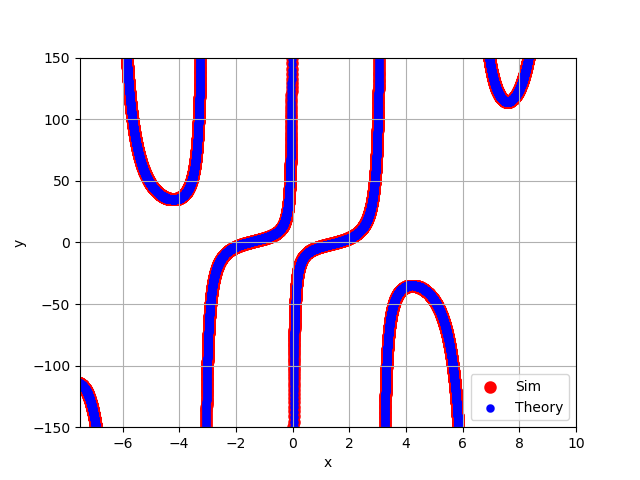
\includegraphics[width=1\columnwidth]{figs/simulated.png}
	\caption{Plot of the solution of $\frac{dy}{dx} + y\cot x = 4x \cosec x$}
	\label{stemplot}
\end{figure}

\end{document}
